\documentclass[a4paper]{article}
\usepackage[T1]{fontenc}
\usepackage[utf8]{inputenc}
\usepackage[italian]{babel}
\usepackage{lipsum}
\usepackage{graphicx}
\author{Anis Lico \and Simone Del Gatto}
\title{Programmazione di reti - Relazione Assigment 3}
\begin{document}
\maketitle



\tableofcontents

\section{Strategie Risolutive}

\subsection{Strutture Dati}
Le strutture dati impiegate per l'implementazione del protocollo richiesto sono le seguenti:
\begin{itemize}

\item \textbf{messToSend}: è una struttura che di permette di realizzare una coda per bufferizzare i messaggi che devono essere inviati da A a B. 

\item \textbf{messagesList}: puntatore alla testa della coda che indica il prossimo messaggio da inviare. Si è deciso di utilizzare una coda in quanto abbiamo considerato che l'idea di utilizzare un buffer limitato a 50 messaggi fosse appunto solo un suggerimento e non un effettiva consegna da rispettare.

\item \textbf{A\_packetBuffer}: array che permette di bufferizzare i pacchetti che A invia a B.

\item \textbf{B\_packetBuffer}: array che permette a B di memorizzare i pacchetti che arrivano disordinati.

\item \textbf{B\_bufferDescriptor}: array che descrive lo stato degli elementi di B\_packetBuffer. Essi possono essere \textbf{EMPTY} che indica che in quella posizione non c'è nessun pacchetto o che il pacchetto che c'è è già stato consegnato da B al layer 5, oppure \textbf{NOT\_SENT\_TO\_5} che indica che il pacchetto in quella posizione deve essere ancora inviato al livello 5 e quindi deve rimanere bufferizzato.

\end{itemize}

\subsection{Descrizione delle Routine}
\begin{itemize}

\item \textbf{A\_init}: inizializza le strutture precedentemente descritte e le variabili utilizzate da A.

\item \textbf{B\_init}: inizializza le strutture precedentemente descritte e le variabili utilizzate da B.

\item \textbf{A\_output(message)}: una volta ricevuto il pacchetto dal livello 5 A controlla tramite un apposito contatore quanti pacchetti sono attualmente nella finestra. Se ci sono ancora posti disponibili nella finestra invia il pacchetto in caso contrario lo aggiunge a \emph{messagesList}. In caso la finestra sia vuota, e ciò avviene quando il numero di sequenza del pacchetto appena inviato è uguale al numero di sequenza del pacchetto che sta alla base della finestra, viene avviato il timer.

\item \textbf{A\_input(packet}: quando A riceve un pacchetto innanzitutto controlla che non sia corrotto(in tal caso il pacchetto viene droppato) e controlla il numero di ack: 

\begin{enumerate}

\item se il numero è al di fuori della finestra vuol dire che quell'ack indica che non ci sono nuovi pacchetti da segnare come correttamente ricevuti da B e quindi non ci sono cambiamenti da fare e il pacchetto viene droppato.

\item il pacchetto ha un numero di acknolegment che si trova all'interno della finestra e quindi tutti i pacchetti fino a quello con il numero di sequenza corrispondente al numero di ack del pacchetto sono stati ricevuti correttamente da B. Viene fermato il timer e si sposta la finestra ponendo come base il numero di sequenza successivo a quello del numero di acknolegment ricevuto. Nel frattempo viene aggiornata la finestra e nel caso ci siano dei posti liberi vengono inviati i messaggi bufferizzati in \emph{messagesList} fino a che o non si svuota il buffer o la finestra non si riempie. Viene poi fatto ripartire il timer.

\end{enumerate}

\item \textbf{A\_timerinterrupt()}: una volta che scatta il timer vengono riinviati tutti i pacchetti presenti nella finestra.

\item \textbf{B\_input(packet)}:  quando B riceve un pacchetto si possono presentare varie casistiche:

\begin{enumerate}
\item il pacchetto ha un numero di sequenza che appartiene alla finestra di B ma non è il pacchetto che si trova alla base di quest'ultima. Il pacchetto viene bufferizzato in \emph{B\_packetBuffer} e viene aggiornato il relativo elemento descrittore del pacchetto nella struttura dati \emph{B\_bufferDescriptor}.
\item il pacchetto ha un numero di sequenza che è quello della base della finestra. Il pacchetto viene consegnato al livello 5 e si controlla se ci sono degli altri pacchetti nel buffer che possono essere consegnati al livello 5 in maniera ordinata. Ogni volta che un pacchetto viene consegnato si aggiorna \emph{B\_bufferDescriptor}.
\item il pacchetto non appartiene alla finestra (si tratta ad esempio di una ritrasmissione di un pacchetto che  però è già stato trasmesso al livello 5) oppure il pacchetto è corrotto: in entrambi i casi il pacchetto viene droppato. 
\end{enumerate}

In tutti i casi viene mandato un ack ad A con un numero di acknolegment uguale al numero di sequenza dell'ultimo pacchetto correttamente ackato.
\end{itemize}
\subsection{Note}
Ovviamente le funzioni utilizzate per l'invio del pacchetti tramite il livello 3 e la consegna dal livello 5 sono quelle fornite dal simulatore come anche quelle utilizzate per la gestione l'avvio e lo stop del timer. Sebbene la richiesta fosse implementare un protocollo selective repeat in cui per ogni pacchetto viene utilizzato un timer per gestire la sua eventuale ritrasmissione, ci è stato impossibile implementare una cosa di questo tipo perché nel simulatore viene fornito un unico timer. Si è scelto come specificato prima di tenere monitorato solo il primo pacchetto della finestra e sarà la mancata ricezione del suo ack relativo a far scattare il timer e a generare una ritrasmissione. Per quanto riguarda i duplicate ack si è deciso che la ricezione di questi ultimi non determinino una ritrasmissione e si è deciso di affidarsi solo alla ritrasmissione generata dal timer.

\subsection{Diagrammi a stati finiti}
Macchine a stati finiti per la descrizione del comportamento dell'entità a e dell'entità B
\begin{figure}[h!]
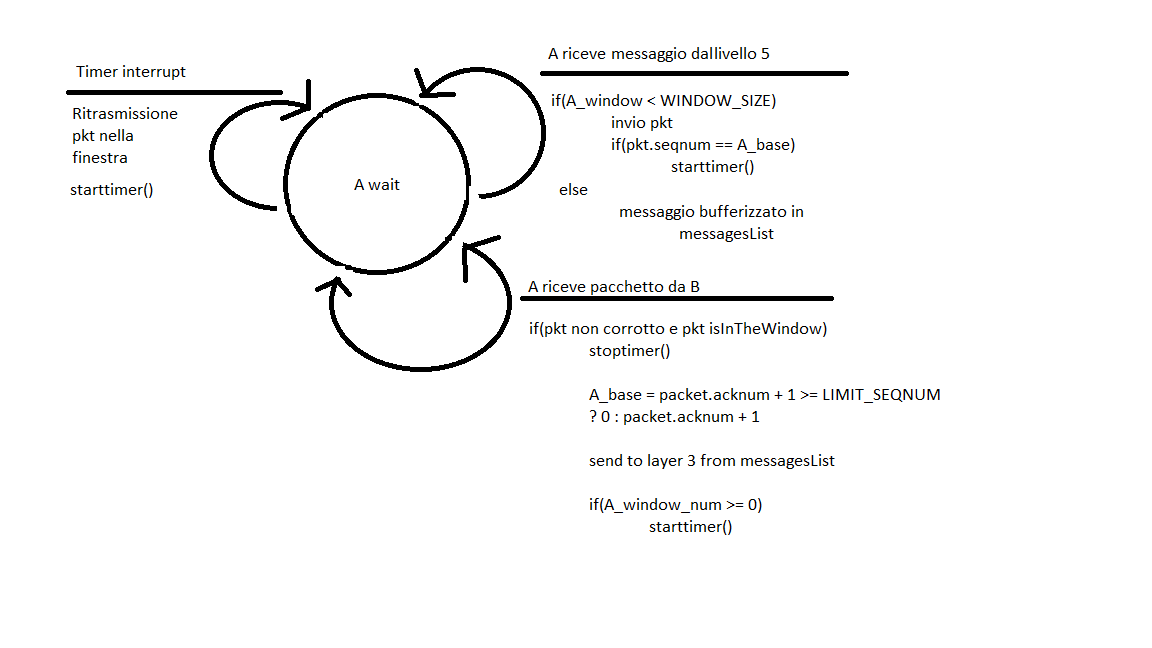
\includegraphics[scale = 0.50]{Assigment3.png}
\caption{Diagramma a stati entità A}
\end{figure}
\newline
\begin{figure}[h!]
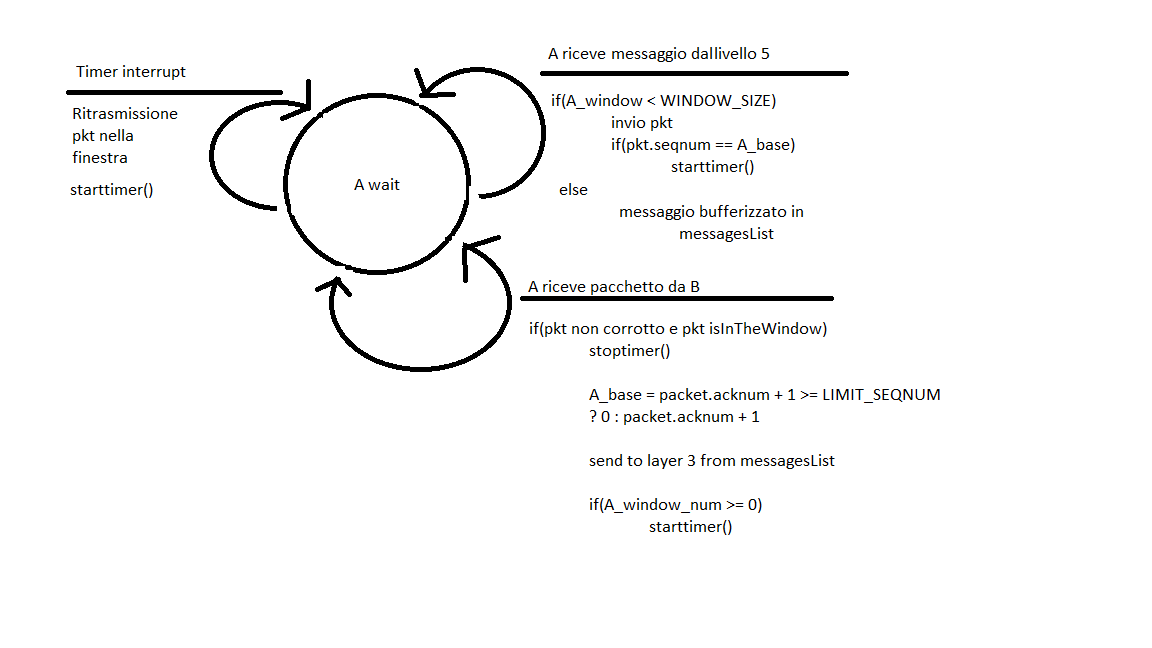
\includegraphics[scale = 0.50]{Assigment3.png}
\caption{Diagramma a stati entità B}
\end{figure}

\section{Test e Relativo output}

\end{document}